%equations, bib. \\
\section{Literature review/State of the art}
There is little specifically helpful literature on the topic of coupled powered systems above and below the surface of the sea. There are however bits and pieces that are useful. Primarily, the offshore oil and gas industry, as well as general ROV operations are able to help a bit. The main issue with this project and its challenges is that it is a form of combined system. There are several papers discussing for instance the effect of currents on deep-submergence suspended tooling used for oil and gas installations. For example, Lian and Sortland 1996 \cite{lian_manoeuvering_1996}. They also performed simulations, however their paper is focused on non-powered remotely operated tooling (ROT) as opposed to a remotely operated vehicle. Their results can be useful as a kind of sanity check for the results of the simulations of this project, though their working area is down to 1500m below the surface while it's improbable that the Plan Sea project will ever operate below 200m. 

The tether is also a consideration for this project, Chen et al. 2021 \cite{chen_dynamic_2021} discuss the hydrodynamic effects on ROV tethers under complex sea conditions. Whether or not this is useful for this implementation is uncertain, as the tether simulations are all done by the simulation software. It might be possible to expand the tether simulations to include Chen et al.'s findings, but this is not done at present. 

Enevoldsen et al., 2018 \cite{enevoldsen_simplified_2018} provide one of the more useful documents on the topic. They discuss a simplified modelling strategy for ROVs to allow for both greater control capabilities and simulated efforts. The state of this project has not used this information, but it will be very helpful in later iterations to expand the accuracy of the simulation for the ROV, both for control purposes and for a more accurate simulation. Anderlini, Parker and Thomas 2018 \cite{anderlini_control_2018} discuss control of an ROV carrying an object. They discuss the sudden added mass of the vessel and how to compensate for it from a control perspective, though their paper focuses more on autonomous underwater maintenance vehicles. This paper as well will be very helpful for further implementation work, but has not been used in any great extent here. Thingstad and Hveding, 1982 \cite{thingstad_nonbuoyant_1982} have a conference paper on non-buoyant ROVs for performing subsea work. On the surface this sounds perfect, but looking into the paper it is more focused on the physical construction of the ROV rather than the control of it. This makes it less helpful for me. Additionally, Thingstad and Hveding's paper is more than 40 years old at time of writing, and applications of control theory, as well as microelectronics and actuators have evolved a lot since then, making what little control they do discuss less useful. Their paper is still mentioned here for completeness.

\section{Mathematical basis}
\label{sec:math}
The root problem can be decomposed into equations \ref{eq:usv} and \ref{eq:rov}. They show the forces that impact the motions of both the surface vessel and the ROV. The forces that have an impact are hydrodynamic forces, such as buoyancy, righting moment etc. The propulsive forces that the vessels' thrusters provide. Environmental forces coming from waves, winds and currents. And finally the force the coupling acts with on each vessel. Do note that though the form of the equations is the same for the surface vessel and the ROV, the values both in total and in each individual element are not going to be equal. Hydrodynamic, propulsive and environmental forces will be entirely individual for each element because of their physical shape and capabilities. The coupling forces however will be linked to each other, though not directly because of how hanging wires act. See \cref{sec:catenary} for elaboration.

\begin{align}
M_{v_{\text{surf}}} = \sum f &= f_{hydro} + f_{prop} + f_{env} + f_ {coupling} \label{eq:usv}\\
M_{v_{\text{ROV}}} = \sum g &= g_{hydro} + g_{prop} + g_{env} + g_ {coupling} \label{eq:rov}
\end{align}

The equations demonstrate the need for simulation compared to analytical examination of the problem. Hydrodynamic forces and environmental forces contribute to a highly dynamic system that is difficult or impossible to find a closed form expression of. This means that calculating an expected state for the dynamic system manually is labour and time intensive. Using a simulation instead of analytical methods hides these problems away. The simulation will take care of the complex interactions which allows me to focus on extracting interesting data. I will further discuss simulation options in \cref{sec:sim_options}

Using a simulation does introduce a new requirement: that of validating the models' accuracy. There are many ways of doing this, both intuitively and mathematically. I will get into these in \cref{sec:validation}. 

The simulation allowing for "setting and forgetting" whatever parts of the force equations are desired allows the user to focus on whatever specific field they are interested in. For example a user might examine the propulsive force required given a certain seastate, or how hull shape and hydrodynamics affects the stability of the total system. 

\subsection{Catenaries}
\label{sec:catenary}
When a rope or chain is suspended from two points and affected by forces not in-line with the two points, the chain forms a catenary. Catenaries are relevant to this project because the lifting tether will form a catenary whenever the ROV is not directly underneath the surface vessel and also in perfectly calm seas. If there is a current affecting the tether it will form a catenary. 

\begin{figure}
	\centering
	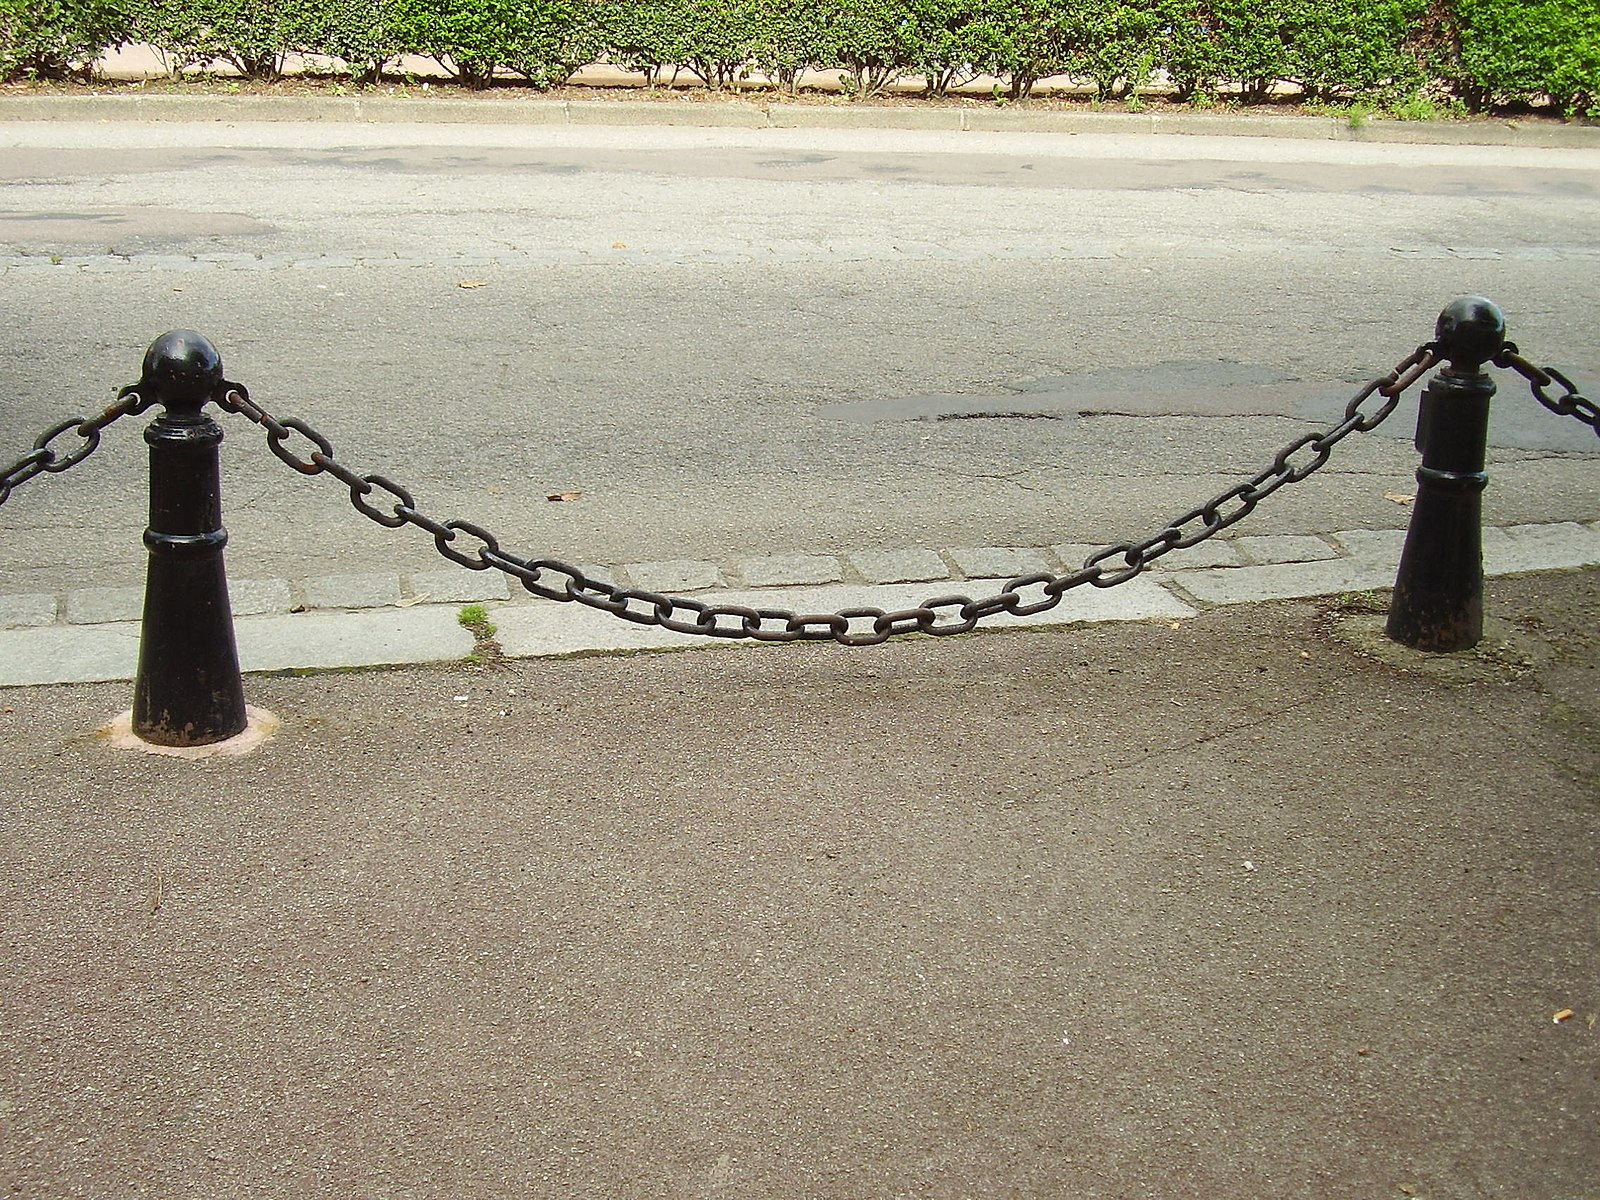
\includegraphics[width=0.6\textwidth]{catenary}
	\caption{A chain forming a catenary between two posts under the force of gravity. Used under Creative Commons, credit: https://en.wikipedia.org/wiki/File:Kette\_Kettenkurve\_Catenary\_2008\_PD.JPG}
	\label{fig:catenary}
\end{figure}

The fact that the lifting tether will form a catenary is helpful to know, as one might intuitively assume that the lifting tether would be straight between the surface vessel and the ROV. If the tether were smooth, finding the position of the ROV could be done by trigonometry, knowing the length of the tether (hypotenuse), its angle at the lifting point relative to gravity, and knowing the tether's azimuth, the ROV could be located. However, since this simplification can't necessarily be done, a slight complication has to be added. The angle at the lifting point is not necessarily directly linked to the angle of a straight line to the ROV. 

In 2 dimensions, a catenary is well defined as 
\[y = a \cosh\left(\frac x a \right)\] 
Where \(a\) defines the width of the catenary and can be found in relation to the relevant forces acting on the rope. For this project's applications however, the shape of the tether can't necessarily be simplified to 2D. I have been unable to find a simple, closed form of the catenary equation in 3D for a rope (as opposed to a plane), though it may well exist. This further solidifies the necessity of a simulation over using analytical methods.

This simulator can be used to find an error between assuming a straight line between the ROV and the surface vessel, compared to the real situation. This error can then be considered to be acceptable or not to be used as a part of positioning the ROV under water.
